\documentclass[tikz,border=3pt]{standalone}
\usepackage[utf8]{inputenc}
\usepackage[T1]{fontenc}
\usepackage{lmodern}
\renewcommand{\familydefault}{\sfdefault}
\usepackage{sansmath}\sansmath
\usepackage{chemfig}
\usepackage{pgfplots}\pgfplotsset{compat=1.18,/pgf/number format/use comma,/pgf/number format/1000 sep={.}}
\usetikzlibrary{arrows.meta,calc,positioning,decorations.pathmorphing,patterns}
% paleta del sitio
\definecolor{nar}{HTML}{E8680C}\definecolor{narc}{HTML}{FFB35C}\definecolor{hielo}{HTML}{FFF3E8}
\definecolor{tinta}{HTML}{1D1D1F}\definecolor{gris}{HTML}{6E6E73}\definecolor{lila}{HTML}{7C5CF0}
\definecolor{azul}{HTML}{2F6FD6}\definecolor{menta}{HTML}{17A673}\definecolor{coral}{HTML}{E8342A}
\begin{document}
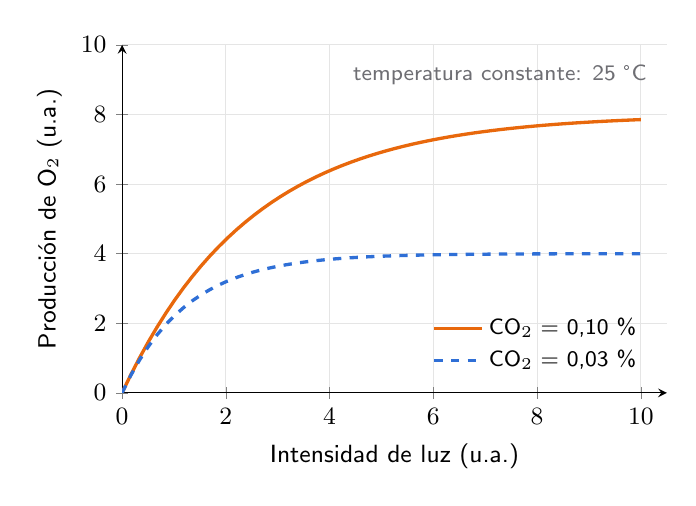
\begin{tikzpicture}[font=\small]
\begin{axis}[width=8.5cm,height=6cm,axis lines=left,xmin=0,xmax=10.5,ymin=0,ymax=10,xlabel={Intensidad de luz (u.a.)},ylabel={Producción de O$_2$ (u.a.)},grid=major,grid style={gray!20},legend style={draw=none,fill=none,at={(0.97,0.03)},anchor=south east,font=\footnotesize},legend cell align=left]
\addplot[nar,very thick,domain=0:10,samples=60] {8*(1-exp(-0.4*x))};
\addlegendentry{CO$_2$ = 0,10 \%}
\addplot[azul,very thick,dashed,domain=0:10,samples=60] {4*(1-exp(-0.8*x))};
\addlegendentry{CO$_2$ = 0,03 \%}
\node[font=\footnotesize,text=gris,anchor=north east] at (axis cs:10.3,9.7) {temperatura constante: 25 °C};
\end{axis}
\end{tikzpicture}
\end{document}
